\documentclass{article}
\usepackage{tikz}
\usetikzlibrary{shapes,shadows,arrows,calc}
\usepackage{pgfplots,pgfplotstable}
\pgfplotsset{compat=1.13}

\usepackage{fp}

\begin{document}
	
	\begin{figure}[ht]
		\centering
		\begin{center}
			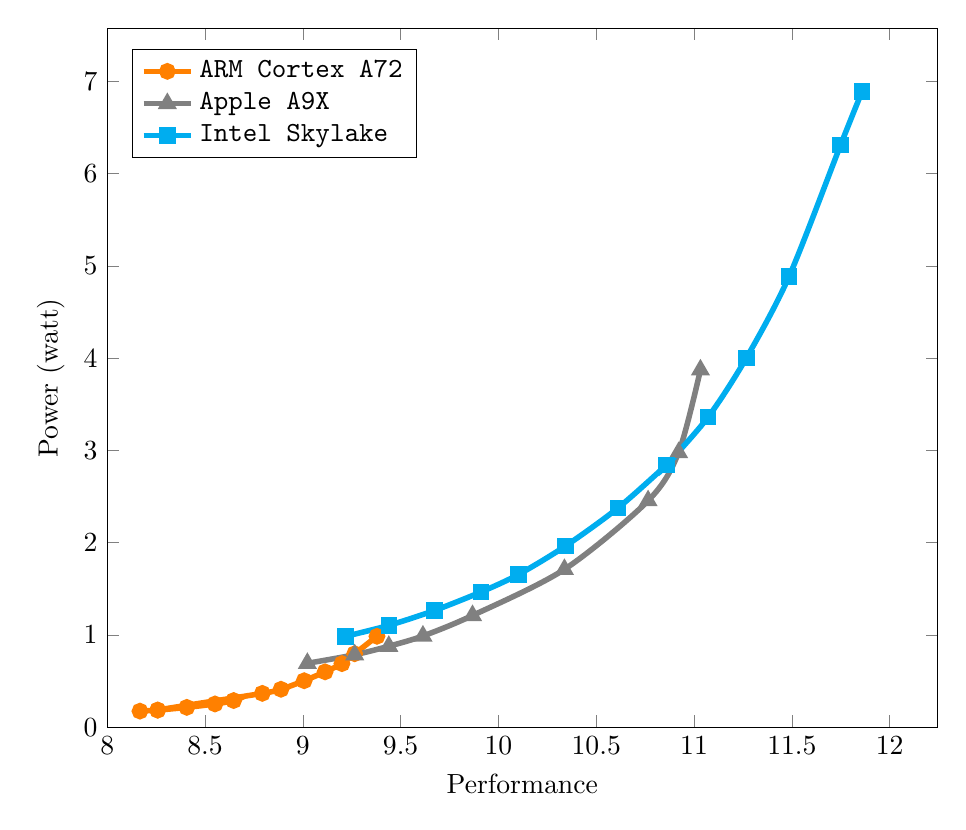
\begin{tikzpicture} %[>=latex]
			\begin{axis}[
			width=1.00\textwidth,
			%line width=2,
			%symbolic x coords={2012, 2013, 2014, 2015, 2016},
			%xticklabels={,,},
			%yticklabels={,,}
			%xticklabels={720p,1080p,4k},
			%minor xtick={0,1,...,18},
			grid=none,
			xmin=8.0,
			ymin=0,
			xlabel=Performance,
			ylabel=Power (watt),
			legend pos=north west,
			legend cell align=left,
			%legend columns=2, 
			legend style={
				fill=none,
			 	%/tikz/column 2/.style={
			 	%	column sep=5pt,
			 	%},
			 },
			%enlarge x limits=0.1,
			%xticklabel style={text width=0.2\textwidth,align=flush left},
			]
			\addplot[line width=2pt,smooth,color=orange,mark=*] coordinates {
				(8+7.2/43,4.7/27) (8+11.1/43,5.0/27) (8+17.5/43,5.8/27) (8+23.7/43,6.8/27) (8+27.8/43,7.8/27) (8+11.1/43,5.0/27) (8+34.1/43,9.9/27) (8+38.2/43,11.1/27)
				(8+43.3/43,13.6/27) (8+47.9/43,16.2/27) (8+51.6/43,18.6/27) (8+54.4/43,21.5/27) (8+59.3/43,26.6/27) %(8+67.1/43,40.5/27)
			};
			\addplot[line width=2pt,smooth,color=gray,mark=triangle*] coordinates {
				(8+44.0/43,18.7/27) (8+54.4/43,21.2/27) (8+61.9/43,23.7/27) (8+69.4/43,26.7/27) (8+80.3/43,32.7/27) (8+100.5/43,46.2/27) 
				 (8+118.9/43,66.3/27) (8+125.6/43,80.4/27) (8+130.4/43,104.6/27) 
			};
			\addplot[line width=2pt,smooth,color=cyan,mark=square*] coordinates {
				(8+52.4/43,26.6/27) (8+61.9/43,29.8/27) (8+72.0/43,34.2/27) (8+82.2/43,39.6/27) (8+90.4/43,44.7/27) (8+100.7/43,53.0/27) (8+112.3/43,64.2/27) 
				(8+123.0/43,76.8/27) (8+123.0/43,76.8/27) (8+132.1/43,90.8/27) (8+140.5/43,108.1/27)  (8+149.9/43,132.0/27) (8+161.2/43,170.4/27) (8+165.9/43,186.0/27)
			};
			\legend{\texttt{ARM Cortex A72}\\\texttt{Apple A9X}\\\texttt{Intel Skylake}\\}
			%\draw[red] plot [smooth] coordinates {(0 0) (2,3700) (4,6006) (18,18000)};
			\end{axis}
			\end{tikzpicture}
		\end{center}
		\caption{Bandwidth required for delivering various videos.}\label{fig:bitrate-resolution}
	\end{figure}
	
\end{document}